\chapter{Design}
\label{chap:Design}

\section{Database}
\label{sec:Database}
The design of the database will look on many points similar to the domain model in figure~\ref{fig:domain_model}. This is because on a lot of the points in this system the domain model can be saved directly to the database. I have of course had to make some adjustments, as can be seen in figure~\ref{fig:Database model}.

\begin{figure}[h]
  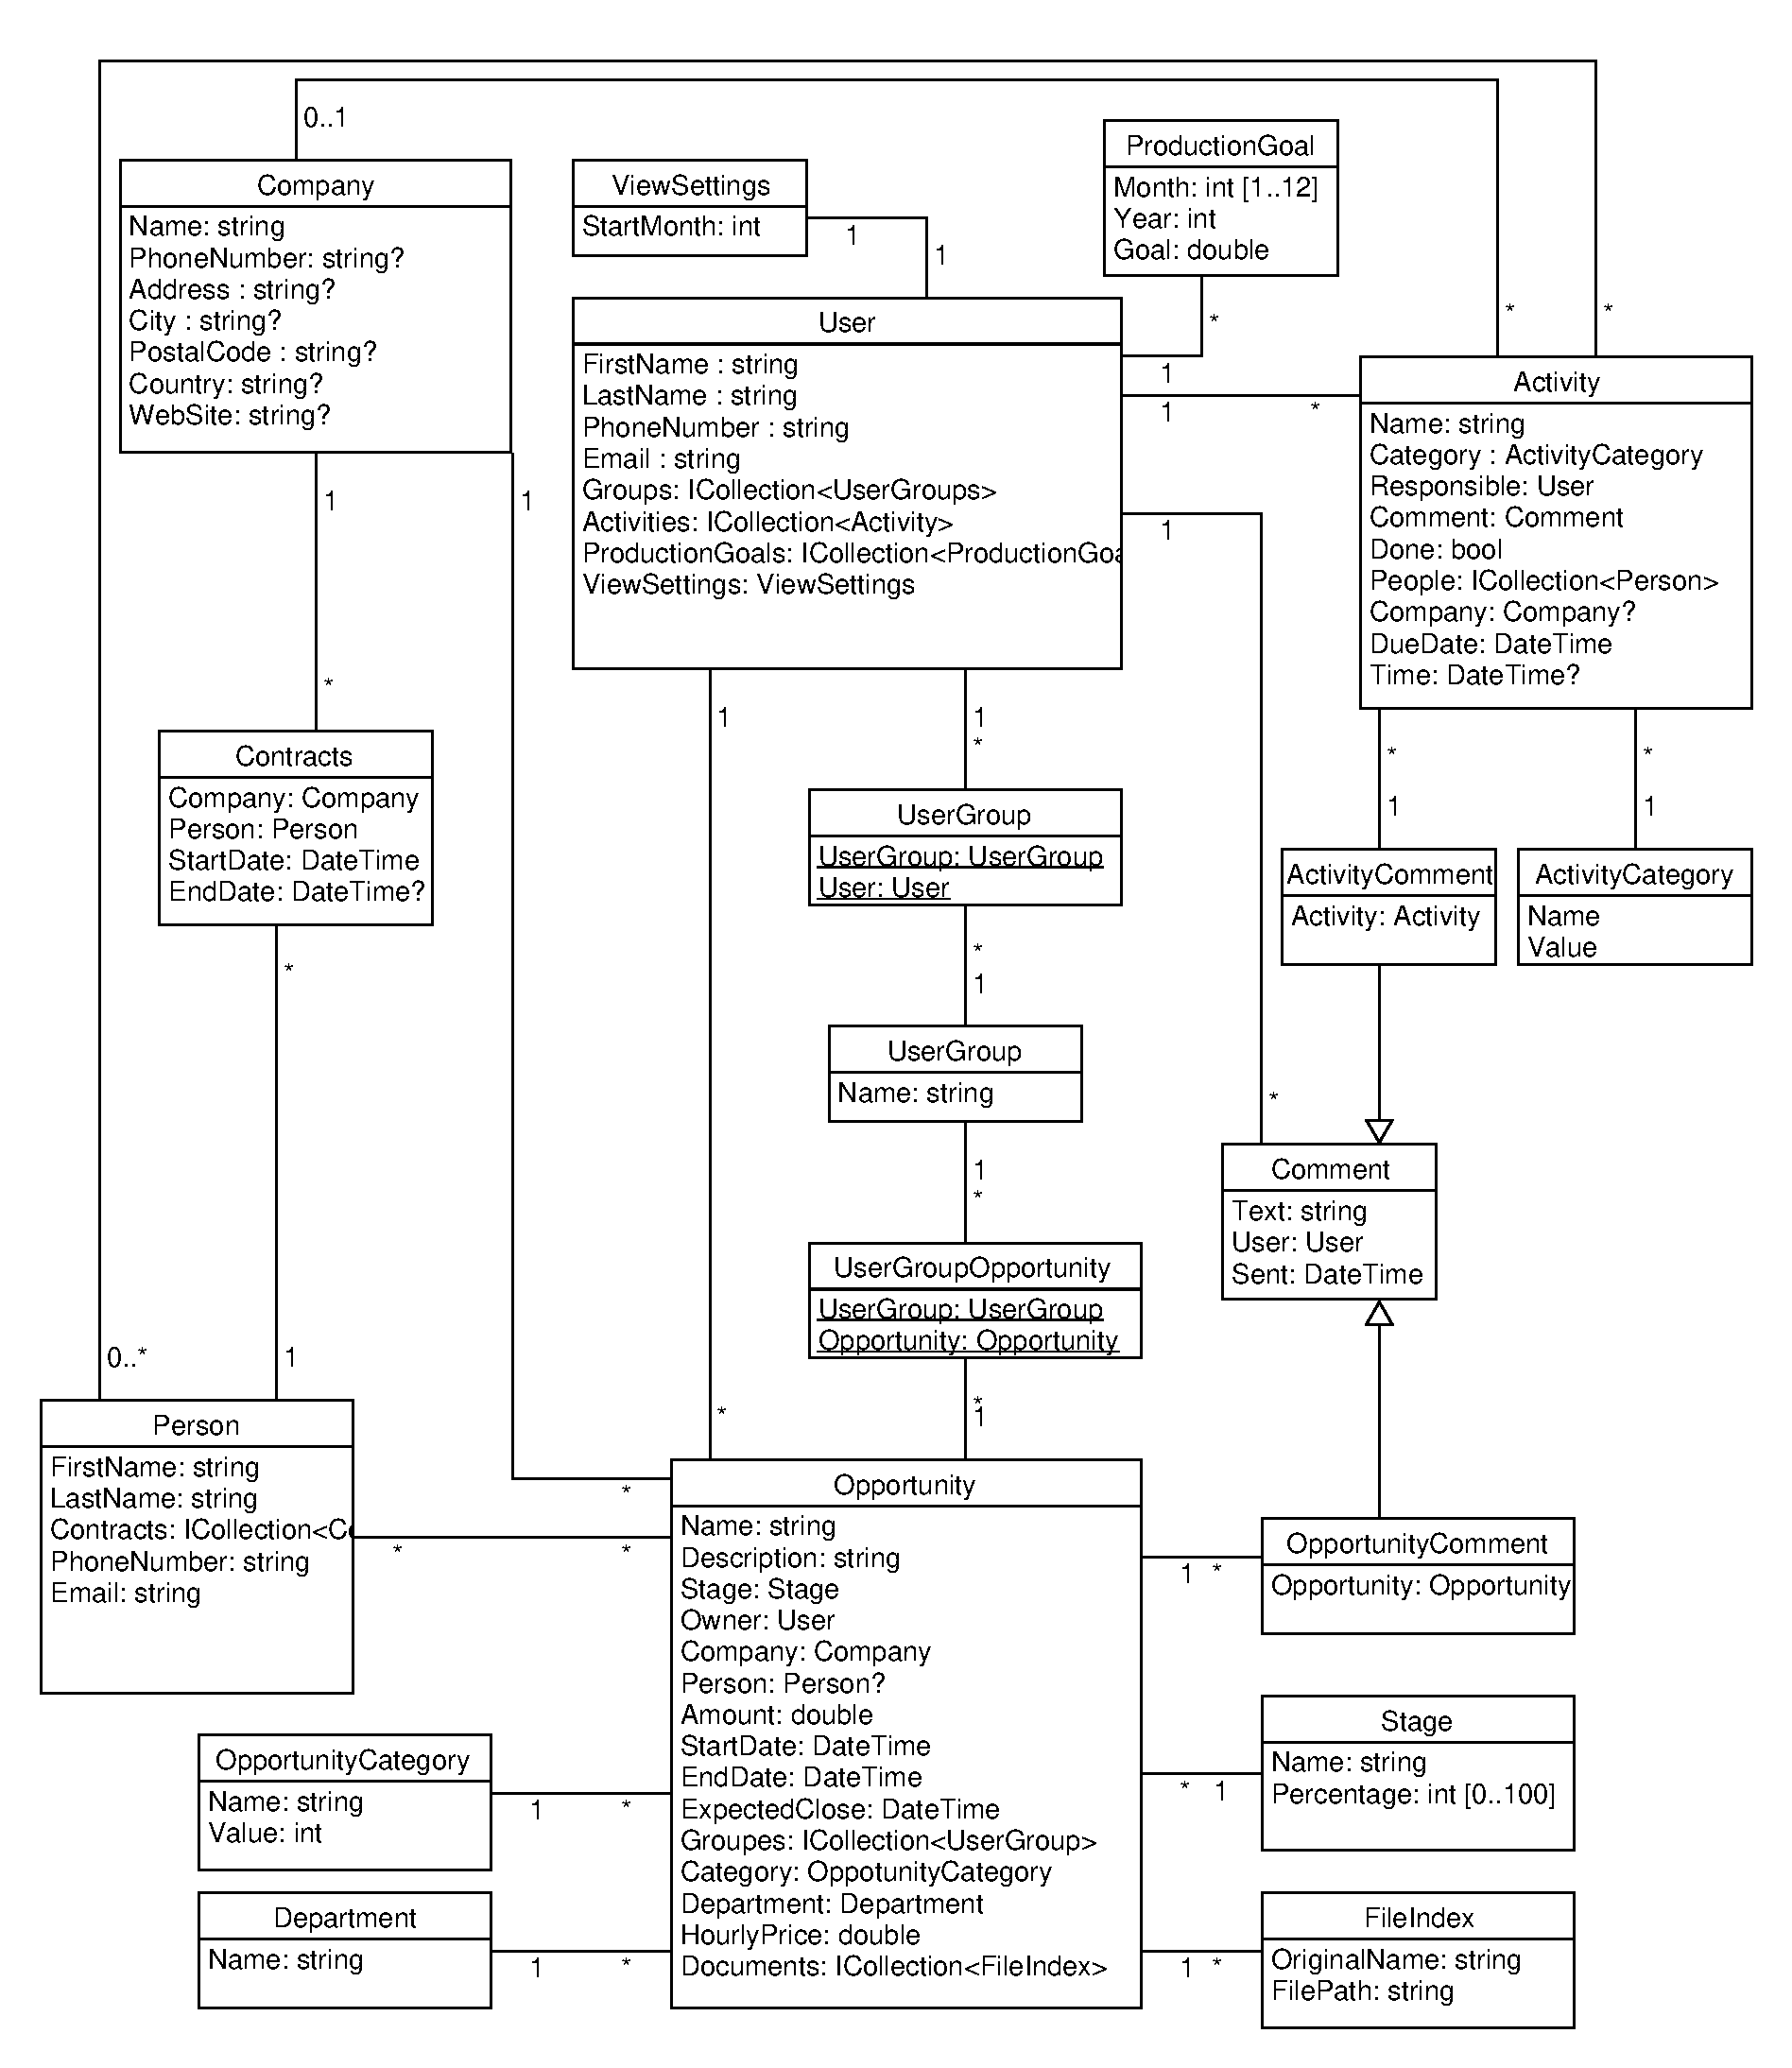
\includegraphics[width=\textwidth]{db_model}
  \caption{Database model}
  \label{fig:Database model}
\end{figure}

One thing that will be noticed is that now we have datatypes on the model. This is because this model is meant to describe what is in the database.

The design is in NF1\footnote{First Normal Form} because we do not have any rows containing any duplicate information, such as a company having a column for all their workers, instead the workers are separated out into a different table\cite[p.~430]{DB_systems}, the same is true for a user and their goals and user groups, instead of having a list of them in the table itself, we have it separated out into different tables.

It is also in NF2\footnote{Second Normal Form} because none of the properties of any of the tables are functionally dependent on anything other than the primary key of the table\cite[p.~434]{DB_systems}. In this case I have not added the primary key to the tables since they will all be called Id as per convention of the entity framework, and I will be giving them an integer as the datatype.\todo{mention i will not alwayse use id as primary key}

The next normal form would be the third normal form. I have come to the conclusion that it is not worth the hassle of perusing this last part as the goal with it is to reduce redundant data to even greater extent, which would mean I would have to move the location based fields of Company out into a separate table in order for me to remove the transitive dependency\cite[p.~436]{DB_systems} there is between the city, address, and postal code, as well as the country. The reason for not pursuing this is that I have deemed the gain not worth it, since it would bind all locations in the same area together, and the users may not be interested in this, since if they then change the postal code or city name of one company, the rest that is located in the same place will follow.

Some people argue that nulls should be allowed and others that there should be no nulls in a database\cite{stackexchange:db:nullfields}, and I do see the reasoning of their arguments, generally that you cannot know what null represents, it could mean the absence of data, purposefully or something else.

One argument is if there is a null value in eg. an integer could mean both null and unknown. A solution to having null values in ones database could be to split it into several tables, one for each potential missing value. I have decided not to do this, since it would make the diagram harder to read, and the database harder to comprehend. Another reason I have chosen not to get rid of all nulls is that I have decided that if a value can be and is null. Then it means that value is not meant to be there. So I will not interpret null as anything but the absence of data.

As an example if we look at the table contracts, the end date can be null, which would mean that there is no end date, and hence the contract is not terminated. If there were an end date however then the termination has been set, maybe in the future, or maybe in the past, that is dependent on the value, but it means that the time of the ended relationship with the company is known.

This forces me to still think about if I should allow a value to e null or not, without forcing me out of the possibility which is why I have chosen that solution.

\section{System structure}
\label{sec:System structure}

\section{Patterns}
\label{sec:Patterns}

\section{Chapter summary}
